\subsection{Experimental setup}
The experiments were executed in a Mac Book Pro with the following characteristics: 2,6 GHz Intel Core i5, 8 GB 1600 MHz DDR3 memory and 256 GB of storage.

\subsection{Analysis}
Data set coming from previous steps are used as an input for the calculations in the analysis. These are some of the most relevant features:
\begin{itemize}
    \item system\_time
    \item cell\_loc
    \item gps\_loc
\end{itemize}

The analysis phase is executed with a following steps:
\begin{enumerate}
    \item Import Parquet data to pySpark DataFrame
    \item Generated and display histograms on pairwise distances
    \item Calculate descriptive statistics on pairwise distances:
        \begin{itemize}
            \item min
            \item max
            \item sum
            \item mean
            \item standard deviation
        \end{itemize}
    \item Calculate Euclidean distance measure on trajectories
    \item Visualize on map
\end{enumerate}

\subsection{Results}
\begin{figure}[h!]
    \centering
    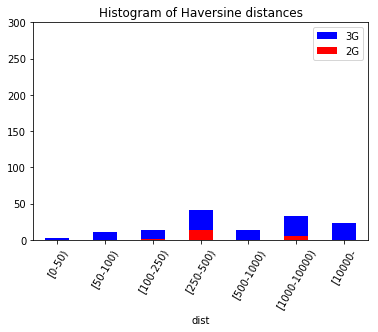
\includegraphics[width=0.45\textwidth]{images/hist_opencell.png}
    \caption{Histogram of distances using OpenCelliD cell map}
    \label{fig:hist_opencell}
\end{figure}

Looking at the histograms of the pairwise Haversine distances between GPS location points and CDR location point on Figure \ref{fig:hist_opencell}, we can say that ???? the majority of the distances fall into the ??? meters range using both cell maps. 

Overall ???\% of the CDR events are positioned with less than ??? meters error. This result can change depending on individual customer's mobile usage habits, network characteristics, cell map data source and the customer's geographical position.

in Table \ref{tab:dist_stats}

\begin{table}[h]
    \centering
    \begin{tabular}{|l|c|}
        \hline 
        count &  \\
        \hline
        Euclidean dist &  \\
        \hline
        min(dist) &  \\
        \hline
        max(dist &   \\
        \hline
        avg(dist) &  \\
        \hline
        stddev(dist) &  \\
        \hline
    \end{tabular}
    \caption{Descriptive statistics of Haversine distances (in meters)}
    \label{tab:dist_stats}
\end{table}

When the user is located between several cell towers, the connection can be passed from one tower to another depending on network traffic fluctuations and other factors. This phenomenon is often referred to as cell tower ping-pong handover. It can however be used for improving positioning and identifying points-of-interest (POIs). As seen in Figure \ref{fig:ping-pong}, the user stays relatively still, but the assigned cell towers change. Without knowing the actual GPS position we can approximate the location of the customer using the ping-pong handover schema.

\begin{figure}[h]
    \centering
    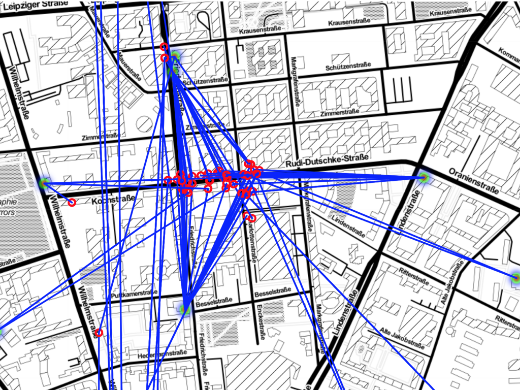
\includegraphics[width=0.5\textwidth]{images/ping-pong.png}
    \caption{Cell ping-pong handover problem}
    \label{fig:ping-pong}
\end{figure}

This method can be further improved if we take into account the angle of the antennas on the cell towers. If we know which antenna is getting the signal, we can guess the direction of the transmitting cell phone and the signal strength can give an approximation of how far away it is. This method is called cell tower triangulation and can be quite accurate in rural regions with more cell towers. However the information about the angles of the antennas and the signal strength can be outdated or even missing therefore it is not always applicable. In this analysis we did not obtain robust data about the positions of the antennas and the signal strength for each CDR event.

Positioning could be improved by reconstructing trajectories considering the road network of Berlin and the potential speed of the movement instead of simply assigning the the cell location from the cell map data.

We identified three major external factors defining the accuracy of the positioning:
\begin{itemize}
    \item individual mobile usage habits affecting the sparsity of CDR data,
    \item geographical location, as rural and urban areas has different cell size and therefore location defines the accuracy of cell tower localization and
    \item cellular network characteristics that define the overall data quality and the available attributes in the CDR data-set.
\end{itemize}


\subsection{Performance tests}
In this section we compare the run-time of the tasks using different Spark standalone clusters and different data sources, namely comma separated value files and Parquet files. The specifications of the clusters are shown in Table \ref{tab:spec}

The selected data-sets for the experiments are:
\begin{itemize}
    \item OpenCelliD data-set: 3.1 GB in .csv  and 1.04GB in Parquet format
    \item CDR data-set: 111KB in .csv and 44KB in Parquet format
\end{itemize}

The operations executed in the experiment are the most common transformations within the project, such as filtering and joining. Since Spark applications are lazily evaluated, a count() operation was called on the resulting DataFrames to reliably reflect the execution time.

\begin{table}[h]
    \centering
    \resizebox{0.45\textwidth}{!}{%
    \begin{tabular}{|l|c|c|}
    	\hline
         & \textbf{Baseline} & \textbf{Alternative} \\
        \hline 
        \# of workers & 1 & 2 \\
        \hline
        Worker cores  & 1 & 1 \\
        \hline
        Worker memory & 1GB & 2GB  \\
        \hline
        Driver memory & 1GB & 1GB \\
        \hline
        Executor memory & 512MB & 1GB\\
        \hline
    \end{tabular}}
    \caption{Specifications of test clusters}
    \label{tab:spec}
\end{table}

Worker memory is the total amount of memory and worker core is the number of cores Spark applications are allowed to use on the machine. Driver memory refers to the amount of memory to use for the driver process, which is where the SparkContext is initialized. Spark executor memory is the amount of memory to use per executor process. %Storage level describes where the RDDs are cached throughout the application's lifetime. Memory refers to the default MEMORY\_ONLY setting, and RDDs are stored as deserialized Java objects in the Java Virtual Machine (JVM). Whenever the RDD does not fit in memory, some partitions will not be cached and will be recomputed on need base. In contrast memory \& disk refers to MEMORY\_AND\_DISK setting, which allows that in case the RDD does not fit in memory, the application can store the non-fitting partitions on disk, and read them from there upon need. 
\cite{spark:rdds}

\subsection{Results}
The execution time of different processing tasks on DataFrame created from the OpenCelliD cell map data-set can be seen in Table \ref{tab:res}.

\begin{table}[h]
    \centering
    \resizebox{0.45\textwidth}{!}{%
    \begin{tabular}{|l||c|c|c|c|}
    	\hline
        \textbf{Task name} & \multicolumn{2}{c|}{\textbf{Baseline}} & \multicolumn{2}{c|}{\textbf{Alternative}}\\
        \hline
        \textit{Data source} & \textit{parquet} & \textit{.csv} & \textit{parquet} & \textit{.csv} \\
        \hline 
        \hline
        read\_data() & 5.27 & 120.68 & 7.19 &  86.6 \\
        \hline
        min\_of\_col() & 3.47 & 65.17 & 4.39 & 44.31 \\
        \hline
        sort\_by\_col() & 25.67 & 158.12 & 29.56  & 107.05 \\
        \hline
        filter\_by\_col() & 2.81 & 67.82 & 4.45  & 46.19 \\
        \hline
        join\_dfs() & 3.66 & 64.05 & 3.15 & 46.06 \\
        \hline
        collect\_rows() & 1.93 & -\footnotemark & 2.12 & -\footnotemark \\
        \hline
        \textbf{Total} & \textbf{42.82} & \textbf{476.84} & \textbf{50.86} & \textbf{330.65} \\
        \hline
    \end{tabular}}
    \caption{Run-times of data processing tasks with different test clusters in seconds}
    \label{tab:res}
\end{table}
\footnotetext{Running collect\_rows() method,'java.lang.OutOfMemoryError: Java heap space' occurs.}
\footnotetext{Running collect\_rows() method,'ConnectionRefusedError' occurs, indicating that an error occurred while trying to connect to the Java server.}

During the experiments we saw that reading data to pySpark DataFrames from Parquet files is more time-efficient than from .csv files, which is in line with our expectations.

The total execution-time in case of Parquet data-source on the Baseline cluster is slightly less then on the Alternate cluster. Since the size of the files is not too large, the benefit of increasing number of workers and their memory could be neutralized by the communication overhead between workers. Instead of adding one more worker, it makes more sense to increase the memory of the existing worker or add more cores. However for large clusters with several physical machines, parallel computation with several workers can be better utilized. Since the test laptop only has 5 cores, adding more than 2 workers is problematic.

In case of .csv data-source the execution time improves by adding another worker and increasing the memory, since the size of the data is larger.

With this architecture design, it is reasonably easy to deploy the application on Amazon Web Services (AWS) or similar cloud service provider allowing scalability to process terabytes of data.